\chapter{Literature study}
\label{chp:litreview}

With the project objectives in mind, we conduct a study of the literature regarding autonomous racing.
Figure \ref{fig:lit_tax_sec} presents a taxonomy of approaches to the solving the autonomous racing problem.
While the majority of efforts fall into the classical or end-to-end categories, a few research efforts have been made into combining classical and end-to-end ideas through a partial end-to-end driving architecture.
Our focus is on examining these various approaches to developing autonomous driving algorithms address the model mismatch and sim-to-real problems.
We end the chapter with a discussion of the research gaps, as well as a summary of the expected contributions of this project towards the literature.

\begin{figure}[htb!]
    \centering
    \input contents/chapt2/figs/literature_taxonomy_sections.tex
    \caption[A taxonomy of the autonomous racing literature]{A taxonomy of approaches to solving the autonomous racing problem. Research efforts associated with each approach are listed.}
    \label{fig:lit_tax_sec}
\end{figure}


\section{Classical approaches}\label{sec:classic}


Classical approaches split the task of generating actuator commands from sensor data into three distinct phases, namely (a) perception, (b) planning and (c) control \cite{Betz2021}.
Perception is the task of processing sensor data into a format that can be used for planning. 
Generally, sensor fusion techniques are used to localise the vehicle within a map \cite{Gotlib2019, Wischnewski2019}.
Planners use the map and localisation data to compute a trajectory that is subject to the vehicle dynamics constraints \cite{Liniger2015a}.
The controller then executes the plan on the physical hardware \cite{Kritayakirana2012}.
This generic framework is illustrated in Figure \ref{fig:full_stack}.

\begin{figure}[h]
    \centering
    \input contents/chapt2/figs/classic_pipeline.tex
    \caption[The classical autonomous driving architecture]{The classical autonomous driving software architecture. The driving software, which is enclosed in the dotted line, maps between sensor input and the commands sent to the actuators by performing perception, planning and control separately.}
    \label{fig:full_stack}
\end{figure}

Classical approaches have successfully been used to control full scale racing cars \cite{Valls2018, alvarez2022, Nekkah2020} at high performance levels and near their handling limits.
For instance, Heilmier et al. \cite{Heilmeier2020} and
Betz et al. \cite{Betz_2023} achieved speeds of $150$ and $270$ km/h respectively.
The success of classical approaches have also been showcased on scaled racing cars by Liniger et al. \cite{Liniger2015}.
We now discuss methods for planning and control in more detail.
Perception algorithms are not discussed because they are outside of the scope for this project.

\subsection{Planning}\label{sec:trajectory_planning}
Within classical approaches, trajectories are generated via optimisation methods that minimise a cost function.
These trajectories trypically consist of a series of $x$ and $y$ coordinates and velocities that must be tracked using controllers.

Several approaches \cite{Heilmeier2020, Kelly2010, Herrmann2019} shift the computational burden of generating a trajectory to offline, before the race starts.
These approaches are categorised by their cost function.
While Heilmeier et al. \cite{Heilmeier2020} optimise the geometry of the path to achieve minimum curvature, Kelly et al. \cite{Kelly2010} considers a time-based optimisation to construct a minimum-time path.
These offline planners create robustness towards the modelling errors by constructing conservative paths and taking vehicle model constraints into account.
For instance, Heilmeier et al. \cite{Heilmeier2020} constrain the curvature of the path so that the vehicle adheres to a maximum lateral acceleration constraint.

While offline planning is useful, a need exists to construct trajectories that actively avoid collisions with the environment or other vehicles in an online manner.
Although it is an optimal control technique, model predictive control (MPC) is commonly used for generating fixed-horizon trajectories online \cite{Liniger2015a, Liniger2015, Anderson2016, Funke2017}.
MPCs sample dynamically feasible trajectories by forward simulating the vehicle dynamics using multiple actuator input sequences.
A cost is assigned to each trajectory, after which the trajectory with the minimum cost is executed \cite{Betz2021}. 
While standard MPCs consider linear vehicle dynamics, Liniger et al. \cite{Liniger2015} proposed a non-linear MPC to more accurately represent the vehicle dynamics.
% They then extended their MPC algorithm by using a viability kernel to characterise every state that leads to a collision on the track, allowing them to sample only safe trajectories \cite{Liniger2015a}. 

Another common approach to constructing a trajectory online is graph based planning, whereby a hierarchical tree of parameterised paths are spanned across the drivable area of the track \cite{Stahl2019, Werling2010, Li2017}.
These approaches calculate the cost of each path based on its geometry, and select the path associated with the least cost.
Since the effect of model-mismatch can be exagurated when extreme control actions are taken, the graph based approach by Stahl et al. \cite{Stahl2019} ensured continuous and smooth paths by parameterising them as cubic polynomials in a curvilinear coordinate frame attached to the track centerline, known as the Frenet frame.
Their method successfully controlled the Devbot $2.0$ Roborace development vehicle shown in Figure \ref{fig:Devbot2} at speeds of up to $212$ km/h.

\begin{figure}[htb!]
    \centering
    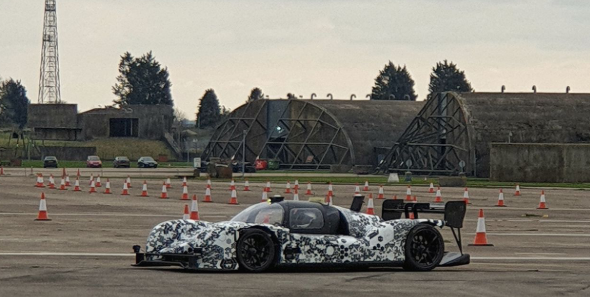
\includegraphics[width=0.7\textwidth]{contents/chapt2/figs/devbot.PNG}
    \caption[The DevBot 2.0 Roborace vehicle]{The DevBot 2.0 vehicle used by Stahl et al. \cite{Stahl2019} in the Roborace. }
    \label{fig:Devbot2}
\end{figure}


\subsection{Control}\label{sec:control}

Controllers allow a trajectory to be executed on hardware by computing control commands that minimise the error between the vehicle's current and desired state.
The use of feedback controllers to follow the trajectory directly addresses the need for robustness towards vehicle model error.
At this level of abstraction, typical control commands are steering angle and longitudinal acceleration, which are sent to low-level controllers to actuate the motors and brakes \cite{Betz2021}.

Classical controllers separate steering and longitudinal acceleration control. 
While longitudinal control is typically performed using a PID controller, methods to perform steering control to track the path vary.
Pure pursuit is a simple steering controller presented by Coulter \cite{Coulter_1992} that steers the vehicle towards a target point on the path that is always some distance ahead of the it.
The steering angles are based on the geometric properties of the vehicle.
Although the method is effective at low speeds, it does not take into account a dynamic model of the vehicle, which leads to sub-optimal performance at higher speeds.

Approaches by Becker et al. \cite{Becker2022} and Hoffman and Montemerlo \cite{Hoffmann2007} also steers the vehicle towards a target point on the path ahead of the vehicle, but compute steering angles based on a dynamic model of the vehicle.
Becker et al. \cite{Becker2022} reported a four-fold improvement in path tracking error over the pure pursuit algorithm on an F1tenth race car, while the controller by Hoffman and Montemerlo \cite{Hoffmann2007} was implemented on the winning vehicle of the DARPA Grand Challenge in 2005.
The vehicle used by Hoffmann et al.  \cite{Hoffmann2007} is shown in Figure \ref{fig:stanley}.

Model predictive control (MPC) is a state of the art classical control technique \cite{Tatulea-Codrean2020, Beal2013, Achin2021, Williams2016, Liniger2019, Brunner2018a}.
When used as a path tracking controller, the objective of the MPC is to minimise the error between the vehicle's actual and planned trajectory \cite{Liniger2019}.
However, many MPC approaches use linearised vehicle models \cite{Beal2013} because the computation requirements for an MPC that utilises a non-linear vehicle model is too demanding for hardware onboard a scaled vehicle to execute \cite{Tatulea-Codrean2020}.
Furthermore, the MPC cost function is considered too inflexible for complex manoeuvres such as racing with multiple vehicles \cite{Fuchs2021}.
% MPCs are also susceptible to modelling errors due to their reliance on accurate vehicle dynamics models \cite{Achin2021}. 
Research efforts into improving the performance of MPCs under model-mismatch conditions are focused on learning a vehicle model online, such that the error between the vehicle model and real vehicle dynamics is minimised \cite{Tatulea-Codrean2020, Brunner2018a}.


\begin{figure}[htb!]
    \centering
    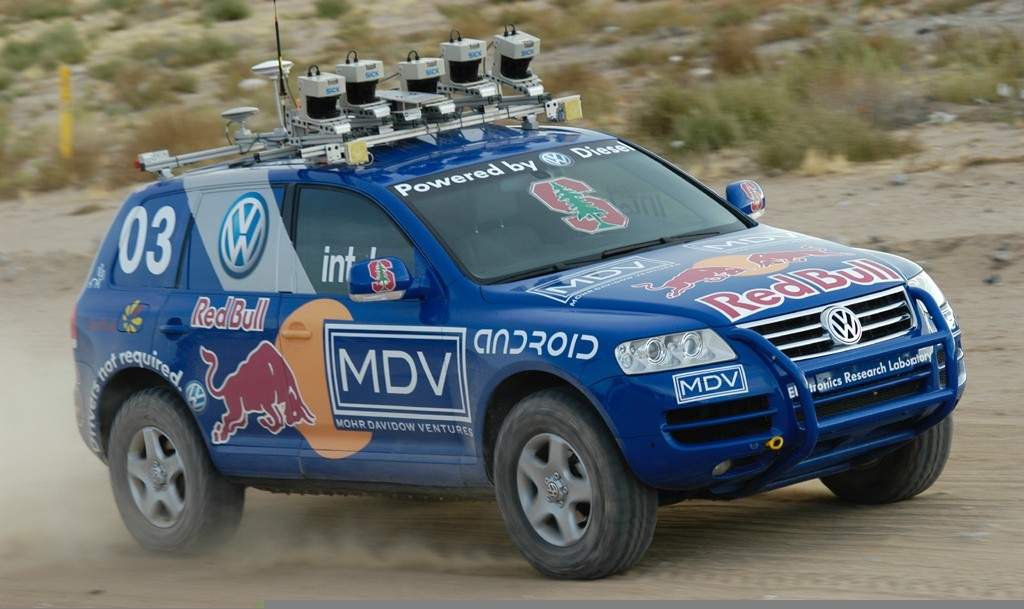
\includegraphics[width=0.5\textwidth]{contents/chapt2/figs/stanley.jpg}
    \caption[The Stanley vehicle]{The controller by Hoffmann et al. \cite{Hoffmann2007} was implemented on a modified Volkswagen Touareg called Stanley. Hoffmann et al.'s vehicle won the DARPA grand challenge in 2005.}
    \label{fig:stanley}
\end{figure}


\section{End-to-end approaches}
\label{sec:end_to_end}

The limitations of optimisation techniques from classical methods has led to research in learning-based systems that use data to formulate a decision-making policy to control the vehicle \cite{Fuchs2021}.
Many learning-based approaches use an end-to-end architecture, whereby a decision making agent, whose policy is typically represented by a deep neural network (DNN), predicts actuator commands directly from sensor data, thus performing the task of the entire classical architecture.
This end-to-end approach is illustrated in Figure \ref{fig:end_to_end}.
The two machine learning paradigms by which the neural networks in end-to-end systems are trained are imitation learning (IL) and reinforcement learning (RL).

\begin{figure}[h]
    \centering
    \input contents/chapt2/figs/end_to_end_pipeline.tex
    \caption[The end to end autonomous driving architecture]{The end-to-end autonomous driving architecture, whereby an agent maps directly from sensor data to actuator commands.}
    \label{fig:end_to_end}
\end{figure}

\subsection{Imitation learning}
\label{sec:imitation_learning}

Imitation learning is a supervised learning technique that aims to learn a mapping from sensor data to control actions, by using examples generated from an expert as training data \cite{Tatulea-Codrean2020, Pan2017a, lee2019, Osa_2018}.
These IL approaches that solve the autonomous racing problem rely on an MPC to provide expert training data.

Tatulea-Codrean et al. \cite{Tatulea-Codrean2020} used an IL algorithm to train a DNN that mimics a non-linear MPC expert. 
Sampling an action from the neural network was less computationally expensive than sampling from the non-linear MPC. 
As such, the use of a DNN made physical deployment tractable given the computational constraints of the F1tenth vehicle that was used as the hardware platform.

The IL approach by Pan et al. \cite{Pan2017a} demonstrated a convolutional neural network (CNN) that is capable of learning a mapping between images taken by a camera mounted to the front of the vehicle, and control actions.
Their approach mimics an MPC expert that has access to a more expensive set of sensors which included a LiDAR.
By using only camera images as input to the CNN, Pan et al. \cite{Pan2017a} were able to circumvent the need for expensive LiDAR sensors.
Furthermore, the IL algorithm performed high speed manoeuvres in a difficult off-road setting where vehicle dynamics modelling inaccuracies are likely to occur due to the difficulty of modelling the track surface.

Lee et al. \cite{lee2019} used IL to to train an ensemble of Bayesian neural networks (BNNs) to create a policy that was robust to sensor failure, which was not possible with previous classical approaches. 
An MPC expert was used to generate training data.
The vehicle and track used by both Lee et al. \cite{lee2019} and Pan et al. \cite{Pan2017a} is shown in Figure \ref{fig:lee_car_track}.

\begin{figure}[htb!]
    \centering
    \begin{subfigure}[htb!]{0.48\textwidth}
        \centering
        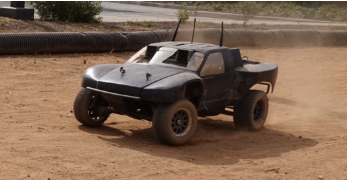
\includegraphics[height=.45\linewidth]{contents/chapt2/figs/IL_car.png}
        \caption[]{}
        \label{fig:IL_car}
    \end{subfigure}
    \hfill
    \begin{subfigure}[htb!]{0.48\textwidth}
        \centering
        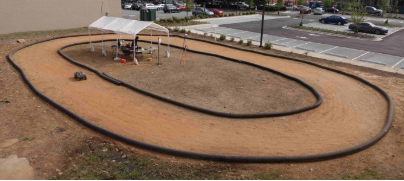
\includegraphics[height=.45\linewidth]{contents/chapt2/figs/IL_track.png}
        \caption[]{}
        \label{fig:IL_track}
    \end{subfigure}
    \hfill
    \caption[The car and track used by Lee et al.]{The (a) $1/5$ scale vehicle and (b) track used by both Lee et al. \cite{lee2019}. and Pan et al. \cite{Pan2017a}.}
\label{fig:lee_car_track}
\end{figure}

The use of end-to-end IL methods necessitates the involvement of an expert MPC to generate the necessary training data \cite{Pan2017}. 
Consequently, the application of IL approaches is restricted to scenarios in which MPCs already demonstrate a high degree of proficiency. 
As such, IL methods do not enhance the sim-to-real capabilities of classical approaches with respect to modeling mismatch. 
Instead, they increase the feasibility of deploying MPC policies on actual vehicles that are subject to computational limitations and potential sensor malfunctions \cite{lee2019, Pan2017}.

\subsection{Reinforcement learning}
\label{sec:reinforcement_learning}
Reinforcement learning is a method that aims to train decision-making agents to maximize a scalar reward signal through direct interaction with their environment \cite{Plaat_2022}. 
In the context of training agents to control racing cars, RL typically uses DNNs to represent the decision-making policy \cite{Betz2021}. 
DNNs offer several advantages when used within an RL framework, including the ability to map complex inputs such as camera images to control outputs \cite{hsu2022, Schwarting2021, Jaritz2018, Perot2017}, as well as the ability to sample actions with low computational cost compared to other methods such as model predictive control \cite{Ghignone2022}. 
Unlike imitation learning (IL) methods, RL algorithms do not require expert training data and can find optimal strategies with minimal human intervention, making them suitable for challenging scenarios such as multi-vehicle racing \cite{Song2021, Wurman2022}. 


\subsubsection*{Reinforcement learning applied to racing video games}

Jaritz et al. \cite{Jaritz2018} and Perot et al. \cite{Perot2017} present research efforts that use model-free RL to train an agent to race in the video game World Rally Championship $6$. 
Model-free RL algorithms enable agents to learn to make decisions based solely on trial and error experience, without using a model of the vehicle or environment.
Both studies focus on RL agents that learn a mapping between the game screen and control output by representing the policy as a CNN with long-short-term memory (LSTM) layers. 
Despite the agents' ability to drive for some distance along the track, Jaritz et al. \cite{Jaritz2018} reported that the vehicle collided with the track boundary an average of 5.44 times per kilometer.

The video game Gran Turismo Sport (GTS) shown in Figure \ref{fig:GTS} has been the subject of several research efforts that showcase model-free RL agents can outperform humans \cite{Song2021, Wurman2022, Fuchs2021} in some race settings.
Fuchs et al. \cite{Fuchs2021} use a DNN to map a hand-crafted set of features to control outputs in a racing scenario where there is a single vehicle on the track.
This agent outperforms even the best competitive GTS players.
Fuchs et al. \cite{Fuchs2021} also considers the effect of model-mismatch on the agent by varying the road-surface friction coefficient after training.
There is significant uncertainty associated with the road-surface friction value due to its dependence on the weather and the difficulty of measuring it at every point along the track \cite{Novikov2018}.
As such, robustness to road-surface friction is a pertinent sim-to-real issue.
However, the agent by Fuchs et al. \cite{Fuchs2021} makes contact with the track boundary when friction varied.

Wurman et al. \cite{Wurman2022} and Song et al. \cite{Song2021} consider GTS racing scenarios with multiple vehicles.
Both approaches achieve better than human performance using a similar set of input features and DNN design as Fuchs et al. \cite{Fuchs2021}.
This demonstrates the ability of RL agents to learn policies that solve complex tasks such as overtaking. 
However, all three approaches that solve GTS allow the vehicle to scrape against the boundary of the track or collide with other vehicles, which is an unrealistic assumption to make for RL agents that are deployed onto physical cars.

\begin{figure}[htb!]
    \centering
    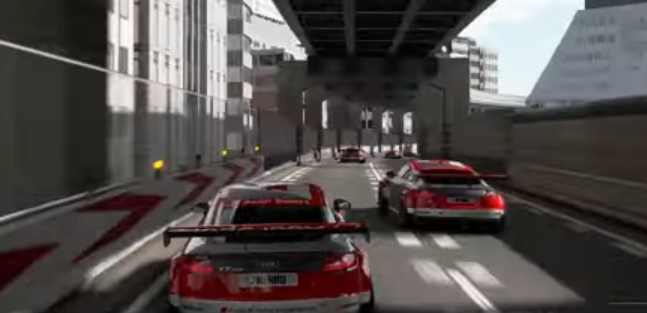
\includegraphics[width=0.6\textwidth]{contents/chapt2/figs/GTS.PNG}
    \caption[An RL agent overtaking multiple vehicles in GTS]{A screenshot of Song et al.'s agent overtaking multiple vehicles in the video game GTS \cite{Song2021}.}
    \label{fig:GTS}
\end{figure}

Cai et al. \cite{Cai2020} present a model-free RL approach to controlling a race car during high-slip drifting manoeuvres in the Speed Dreams simulator.
The agent controls the vehicle beyond the friction limit of the tires.
While their approach demonstrates that RL agents can learn to control vehicles with complex non-linear dynamics, their DNN maps an unrealistic set of input features (e.g., the derivative of the angle between the vehicle's heading and forward velocity vector) to control actions. 

RL techniques have shown excellent performance when applied to racing games. 
However, these approaches make unrealistic assumptions that render them infeasible for real-world driving scenarios.
The most significant challenges to applying these approaches on physical vehicles are the lack of safety considerations and the availability of unrealistic input features sets.


\subsubsection*{Reinforcement learning applied to realistic racing scenarios}
The following approaches have either been deployed on physical hardware, or make realistic enough assumptions to be applied to physical hardware.
The focus is on techniques that improve the sim-to-real capabilities of RL agents.

Niu et al. \cite{Niu2020} address the issue that DNNs do not have perfect prediction accuracy and can select unsafe actions that lead to crashes, even after deployment.
Their approach uses a model-based safety controller that acts as a safeguard mechanism to prevent the agent from selecting unsafe actions on a vehicle simulated with the open racing simulator (TORCS).
Their model-free RL agent did not crash during training or testing with the safeguard mechanism in place.
Niu et al.'s \cite{Niu2020} approach may alleviate the sim-to-real gap by allowing an RL agent to train directly on the physical hardware without risking a crash. 
However, their approach is not validated on a physical vehicle.

The effectiveness of model-based RL in real-world applications is demonstrated by Brunbauer et al. \cite{brunnbauer2021}, who deploy an agent which learns to control the physical F1tenth vehicle shown in Figure \ref{fig:brunbauer}.
\begin{figure}[htb!]
    \centering
    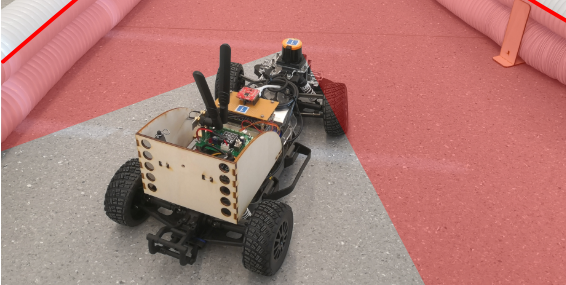
\includegraphics[width=0.6\textwidth]{contents/chapt2/figs/brunnbauer.PNG}
    \caption[The F1tenth vehicle used by Brunbauer]{The F1tenth vehicle used by Brunbauer et al. \cite{brunnbauer2021}. The red area indicates the field of view of the LiDAR scanner on the vehicle.}
    \label{fig:brunbauer}
\end{figure}
Their agent learns to race using the Dreamer algorithm \cite{Hafner2019a}, whereby a learned observation model is used to predict agent-track interactions.
The agent can then learn a policy based purely on `imagined' sequences using the observation model, without interacting with the track.


Hsu et al. \cite{hsu2022} deployed a model-free RL agent that takes camera images as input onto a physical F1tenth vehicle.
They apply conditioning for action policy smoothness (CAPS) \cite{Caps2021} as a policy output regularisation strategy.
Policy output regularisation aims to prevent  jerky and extreme vehicle control actions by adding the difference between actions selected on consecutive time steps to the cost function of the policy update.
% Reinforcement learning agents are known to take extreme control actions, such as swerving the race car unnecessarily to the left or right \cite{Brunnbauer2021a, Ghignone2022}.
Extreme steering and acceleration control actions causes the vehicle to operate closer to the friction limits of the tires than with smooth control actions, and can lead to uncontrollable and dangerous behaviour.
This issue becomes more pertinent when considering scenarios in which model mismatches are present \cite{Chisari2021}.

Hsu et al. \cite{hsu2022} also employed domain randomisation by adding noise to the input camera images.
Domain randomisation involves varying the simulation environment slightly during training.
This prevents the agent from forming a policy that overfits to a single simulation environment.
Moreover, it is more likely that the data encountered by the agent during training includes the distribution of data encountered after deployment when domain randomisation is used \cite{Zhou2020}.
The standard end-to-end agent's average lap completion rate, along with agents trained using solely policy output regularisation or solely domain randomisation was $0\%$. 
However, average lap completion rate increased to $42\%$ when both domain randomisation and policy output regularisation techniques were used.

Ivanov et al. \cite{Ivanov2020} trained a model-free RL agent to steer the F1tenth  vehicle  shown in Figure \ref{fig:ivanov} around a corner using only a LiDAR sensor as input.
They identified their perception model (i.e., the simulated LiDAR sensor) as a major source of uncertainty because the track reflectivity was unknown.
Although they applied domain randomisation techniques by randomising LiDAR measurement noise, they achieved an $83\%$ success rate rounding the corner using their best method.

\begin{figure}[htb!]
    \centering
    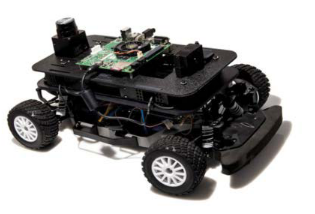
\includegraphics[width=0.3\textwidth]{contents/chapt2/figs/ivanov.PNG}
    \caption[Ivanov's F1tenth vehicle]{Ivanov et al.'s F1tenth vehicle \cite{Ivanov2020}.}
    \label{fig:ivanov}
\end{figure}


Chisari et al. \cite{Chisari2021} also utilized domain randomisation and action smoothing techniques to enable a model-free RL agent to control 1:43 scale cars in their study. 
Rather than adding noise to the sensor readings, they apply domain randomisation by adding noise to the vehicle dynamics model parameters.
Without domain randomisation, the agent was unable to complete even a single lap on the physical car. 
When they compared their baseline reinforcement learning agent which incorporated only domain randomisation to an MPC, the MPC outperformed their agent in terms of both lap time and track boundary violations. 
However, their agent that used domain randomisation and output policy regularization demonstrated a $30\%$ reduction in track boundary violations compared to the MPC method, although it had an $8.1\%$ slower lap time.

Table \ref{table:autonomous_racing_rl_summary} summarizes the end-to-end RL approaches reviewed. 
While these algorithms have delivered impressive results in simulation, practical implementations have been limited to small-scale vehicles,
primarily using the F1tenth racing platform. 
Furthermore, results have shown that end-to-end agents often fail under model-mismatch conditions.

\newcolumntype{R}{>{\raggedleft\arraybackslash}p{2.7cm}}
\newcolumntype{M}{>{\centering\arraybackslash}p{1.8cm}}
\newcolumntype{N}{>{\centering\arraybackslash}p{2.2cm}}
\newcolumntype{Y}{>{\centering\arraybackslash}p{1cm}}
\newcolumntype{L}{>{\raggedright\arraybackslash}p{7cm}}


\begin{table}[htb!]
\centering
\renewcommand{\arraystretch}{1.5}
%\resizebox{\textwidth}{!}{
\begin{tabularx}{0.9\textwidth}{R Y M L}
    \hline
    \small \textbf{Author(s)} & \small \textbf{Year} & \small \textbf{Physical \mbox{vehicle}} & \small \textbf{Sim2real research contribution} \\
    \hline
   
    \small Jaritz et al. \cite{Jaritz2018} & \small 2018 & & - \\

    \small Perot et al. \cite{Perot2017} & \small  2017 & & - \\

    \small Fuchs et al. \cite{Fuchs2021} & \small 2021 & & \small Test effects of model inaccuracy in simulation. \\

    \small Song et al. \cite{Fuchs2021} & \small 2021 & & - \\

    \small Wurman et al. \cite{Wurman2022} & \small 2021 & & - \\

    \small Cai et al. \cite{Cai2020} & \small 2021 & & - \\

    \small Niu et al. \cite{Niu2020} & \small 2020 & & \small Safety module based on learned vehicle model prevents agent from selecting unsafe actions. \\
    
    \small Brunnbauer et al. \cite{brunnbauer2021} & \small 2021 & F1tenth & - \\

    \small Hsu et al. \cite{hsu2022} & \small 2022 & F1tenth & \small Domain randomisation while training. Control action smoothing. \\

    \small Ivanov et al. \cite{Ivanov2020} & \small 2020 & F1tenth & \small Domain randomisation while training. \\

    \small Chisari et al. \cite{Chisari2021} & \small 2021 & $1:43$ scale cars & \small Domain randomisation while training, policy refinement after deployment. Control action smoothing.\\

    \hline

\end{tabularx}
%}
\caption[A summary of end-to-end reinforcement learning approaches for autonomous racing]{A summary of end-to-end reinforcement learning approaches for autonomous racing. }
\label{table:autonomous_racing_rl_summary}
\end{table} 



\section{Partial end-to-end approaches}
\label{sec:partial_end_to_end}

Approaches to designing autonomous driving algorithms that synthesise the classic and end-to-end techniques are now considered. 
In these approaches, the modular structure of classic approaches are utilised.
However, rather than implementing techniques associated with classic approaches in each of the modules, the modules may be combined with or replaced by a DNN.
Two popular partial end-to-end design philosophies are to use a DNN to perform the task of the planner \cite{Capo2020, Weiss2020, Weiss2020a, Mahmoud2020}, or the task of the controller \cite{Ghignone2022, Evans2021b}.
The resulting driving software architectures are shown in Figure \ref{fig:pete}.

\begin{figure}[htb!]
    \centering
    \begin{subfigure}[htb!]{\textwidth}
        \centering
        \input contents/chapt2/figs/partial_end_to_end_learned_control.tex
        \caption[]{}
        \label{fig:pete_learned_control}
    \end{subfigure}
    \hfill
    \begin{subfigure}[htb!]{\textwidth}
        \centering
        \input contents/chapt2/figs/partial_end_to_end_learned_planning.tex
        \caption[]{}
        \label{fig:pete_learned_trajectory_planning}
    \end{subfigure}
\caption[Configurations of the partial end-to-end pipeline]{The two configurations of the partial end-to-end pipeline are (a) a classic planner in conjunction with a learned controller, and (b) a learned planner in conjunction with a classic controller. Both configurations require a perception module to localise the vehicle.}
\label{fig:pete}
\end{figure}



\subsection{Learned controller}
\label{sec:learned_controller}
In the partial end-to-end configuration with a learned controller, 
the autonomous driving system leverages classical perception and planning algorithms. 
In this setup, a DNN serves as the controller by learning mapping between the vehicle's current state and desired state to issue actuator commands \cite{Betz2021}.

Evans et al. \cite{Evans2021b}, used an RL agent to modify the control output of a pure pursuit path follower that tracks a global path, with the goal of avoiding previously unseen obstacles on the track.
Their experiments were performed on a simulated F1tenth setup.
The proposed partial end-to-end agent is able to avoid $94\%$ of unseen obstacles without maintaining an obstacle map, while maintaining a smoother path than the baseline end-to-end agent.

In a study by Ghignone et al. \cite{Ghignone2022}, a simulated F1tenth vehicle's path tracking controller was replaced with a model-free RL agent. 
During training, domain randomisation was applied by varying the tire friction coefficient. 
The results showed that the approach led to $6.7$-fold and $2.7$-fold improvements in the number of track collisions under model-mismatch conditions compared to an end-to-end agent and a classical MPC approach, respectively. 
Figure \ref{fig:TC} showcases the performance difference between the end-to-end and partial end-to-end agents by displaying the paths taken by both agents rounding a corner multiple times.
The partial end-to-end agent visibly swerves less and collides with the track boundary fewer times than the end-to-end agents.
These findings demonstrate the benefits of decoupling the planning and control tasks for learning-based systems. 
Specifically, decoupling planning and control in learning-based systems can enhance their robustness towards model mismatch - similar to classical approaches.

\begin{figure}[htb!]
    \centering
    \begin{subfigure}[htb!]{0.49\textwidth}
        \centering
        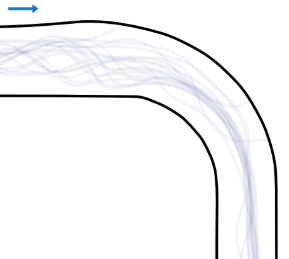
\includegraphics[height=.45\linewidth]{contents/chapt2/figs/TC_end_to_end.png}
        \caption[]{}
        \label{fig:TC_end_to_end}
    \end{subfigure}
    \hfill
    \begin{subfigure}[htb!]{0.49\textwidth}
        \centering
        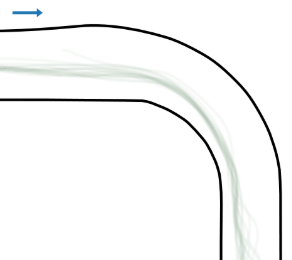
\includegraphics[height=.45\linewidth]{contents/chapt2/figs/TC_partial.png}
        \caption[]{}
        \label{fig:TC_partial}
    \end{subfigure}
    \hfill
    \caption[Distributions of paths taken by end-to-end and partial end-to-end agents]{Distributions of paths taken by (a) an end-to-end and (b) a partial end-to-end agent to round a corner multiple times during an experiment by Ghignone et al. \cite{Ghignone2022}.}
\label{fig:TC}
\end{figure}

\subsection{Learned trajectory planner}
\label{sec:learned_planner}

In a partial end-to-end configuration with a learned planner, the autonomous driving system uses classical perception and control algorithms in conjunction with a deep neural network (DNN). 
The DNN is trained to map perception data (i.e., vehicle state and track information) to trajectories. 
These trajectories are then tracked by classical controllers, enabling the vehicle to race autonomously \cite{Betz2021}.

Weiss and Behl \cite{Weiss2020, Weiss2022} conducted an extensive examination of partial end-to-end systems in which a deep neural network (DNN) replaces the planner. 
Specifically, they utilized an IL algorithm to train a DNN to generate trajectories that were tracked using a pure pursuit controller. 
They applied this approach to a realistic Formula One (F1) video game, which allowed them to use human experts playing the video game as training data.
Through experimentation, they discovered that generating trajectories using B\'ezier curves resulted in high performance. 
Their proposed partial end-to-end method significantly outperformed the end-to-end baseline agent. 
In particular, the end-to-end agent was unable to finish a lap without crashing, while their approach successfully completed laps.

Capo et al. \cite{Capo2020} employed a model-free RL agent to learn the task of planning in the TORCS simulator. 
Specifically, the agent was trained to produce a single point in front of the vehicle, given a hybrid input consisting of a bird's-eye view of the car as well as the vehicle's state. 
This approach exhibited significant improvement over end-to-end agents. 
Capo et al. \cite{Capo2020} explain that this outcome is unsurprising since the partial end-to-end system has embedded driving knowledge via the low-level controller. 
However, the assumption that a bird's-eye view of the vehicle is available is unrealistic for deployment on a physical vehicle.

Table \ref{table:autonomous_racing_partial_end_to_end_summary} presents a summary of the partial end-to-end methods reviewed. 
While partial end-to-end systems have shown superior performance compared to end-to-end systems in simulation, their performance on physical cars is yet to be evaluated. 
Furthermore, there are relatively few research efforts into partial end-to-end systems compared to end-to-end approaches.


\newcolumntype{R}{>{\raggedleft\arraybackslash}p{2.7cm}}
\newcolumntype{M}{>{\centering\arraybackslash}p{1.8cm}}
\newcolumntype{N}{>{\centering\arraybackslash}p{2.2cm}}
\newcolumntype{Y}{>{\centering\arraybackslash}p{1cm}}
\newcolumntype{L}{>{\raggedright\arraybackslash}p{4.5cm}}

\begin{table}[htb!]
\centering
\small
\renewcommand{\arraystretch}{1.1}
\begin{tabularx}{0.9\textwidth}{RYMNL}
    \hline
    \small \textbf{Author(s)} &  \small \textbf{Year} & \small \textbf{Learning method} & \small \textbf{Learned component} & \small \textbf{sim2real approach} \\
    \hline
    \small Weiss and Behl \cite{Weiss2020, Weiss2020a, Weiss2022} & \small $2020$ & \small IL & \small Planner  & - \\
    \small Capo et al. \cite{Capo2020} & \small $2022$ & \small RL &  \small Planner & - \\
    % \small Mahmoud et al. \cite{Mahmoud2020} & \small $2020$ & \small RL & \checkmark & & - \\
    \small Evans et al. \cite{Evans2021b} & \small $2021$ & \small RL &  \small Controller & - \\
    \small Ghignone et al. \cite{Ghignone2022} & \small $2022$ & \small RL &  \small Controller  & \small Randomise vehicle model parameters while training \\
    \hline
\end{tabularx}
\caption[A summary of partial end-to-end approaches for autonomous racing]{A summary of partial end-to-end approaches for autonomous racing.}
\label{table:autonomous_racing_partial_end_to_end_summary}
\end{table} 



\section{Evaluation of existing approaches}

Classical approaches lead learning-based approaches in terms of real-world driving capabilities.
The fact that several classical approaches achieve high speed control of full-size physical vehicles indicates that they are robust towards model mismatches and the sim-to-real transfer \cite{Stahl2019,Betz2019}.
This robustness is achieved through the decoupling of planning and control tasks. 
Furthermore, both planners and controllers are designed to account for uncertainty in the vehicle dynamics.
Planners are designed to generate trajectories that conform to the physical constraints of the vehicle \cite{Heilmeier2020, Kelly2010, Stahl2019}. 
Meanwhile, controllers are responsible for ensuring robustness to model-mismatch by guiding the vehicle towards the trajectory determined by the planner using feedback loops \cite{Coulter_1992, Becker2022, Hoffmann2007}.
Additionally, a recent research trend is improving the vehicle dynamics model online, so that the modelling error is eliminated \cite{Tatulea-Codrean2020, Brunner2018a}.

In contrast, many learning-based and RL systems are implemented in an end-to-end manner.
Furthermore, a significant portion of research in the area of end-to-end RL has focused on model-free techniques for training the agent, 
which excludes the possibility of enhancing the policy by learning an accurate vehicle model online like classical approaches.
Instead, the general approach taken by end-to-end RL methods to increase robustness towards model mismatch is to 
introduce slight variations to the simulation used during the training process using domain randomisation \cite{Ivanov2020, hsu2022, Chisari2021}.

An effective strategy for domain randomisation is to introduce noise to the vehicle parameters \cite{Chisari2021}. 
However, the optimal policy is highly sensitive to the vehicle model parameters, especially those pertaining to the road surface friction. 
As such, the policy discovered through domain randomisation is likely to be suboptimal for most scenarios.
Domain randomisation was also commonly used in conjunction with policy output regularisation to smooth the control actions \cite{hsu2022, Chisari2021}.
However, approaches that employ these techniques \cite{Ivanov2020, hsu2022, Chisari2021} still violate track boundaries, indicating that they do not guarantee the safety of the vehicle.

Partial end-to-end systems present a promising solution for increasing robustness towards model-mismatch by utilising the decoupled structure of classic approaches
For instance, Ghigone et al. \cite{Ghignone2022} showed that their learning-based system exhibited excellent robustness to model-mismatch by training an RL agent to learn the task of the controller. 
However, the advantages of learning-based systems are their ability to learn complex behavior, and relegating the RL agent to the task of path following largely negates this benefit. 
Furthermore, classical controllers can reliably achieve path following \cite{Coulter_1992, Becker2022, Hoffmann2007}.

Several partial end-to-end approaches \cite{Capo2020, Weiss2020, Weiss2020a, Weiss2022} have utilized a partial end-to-end structure whereby an RL agent is used for planning in conjunction with a classic controller for path tracking. 
These systems benefit from the agent's heuristic while constructing the plan, while also leveraging the reliability of classical controllers to follow the path \cite{Betz2021}.
These systems have consistently outperformed end-to-end systems by a significant margin in simulation studies. 
However, their results have not been validated under conditions where model mismatches are present. 
Thus, a research gap exists to determine whether a partial end-to-end system that includes a learned planner and a classic controller can offer better performance under model-mismatch conditions than current learning-based systems.

To determine whether the performance of current common RL (i.e., end-to-end) systems can be improved by combining an RL planner and classic controller in a classic algorithm structure,
the thesis will cover the theoretical foundations of RL agents, the development and implementation of a partial end-to-end system, as well as an end-to-end system. 
Furthermore, our work will compare the performance of these two systems under practical model-mismatch conditions. 
This research seeks to contribute to the existing literature by providing insight into the potential benefits of using partial end-to-end systems over current end-to-end systems.




% \section{Expected contributions}
% Current learning-based approaches lack the incorporation of insights from classical approaches to create algorithms that are robust to model-mismatch. 
% While classical approaches decouple the planning and control tasks, learning-based systems are most commonly implemented end-to-end. 
% Although there are some research efforts into partial end-to-end systems that decouple planning and control, the idea of utilizing classical controllers within a partial end-to-end system to increase robustness towards model-mismatch is a gap in the literature that the authors aim to address.

% To determine whether the performance of current learning-based (i.e., end-to-end) systems can be improved by combining an RL planner and classic controller,
% the thesis will cover the theoretical foundations of RL agents, the development and implementation of a partial end-to-end system, as well as an end-to-end system. 
% Furthermore, our work will compare the performance of these two systems under practical model-mismatch conditions. 
% This research seeks to contribute to the existing literature by providing insight into the potential benefits of using partial end-to-end systems over current end-to-end systems.

